% Copyright (C) Tanner Koza - All Rights Reserved
% Unauthorized copying of this file, via any medium is strictly prohibited
% Written by Tanner Koza <jtk0018@auburn.edu>, October 2022

\documentclass[12pt,letterpaper, onecolumn]{exam}
\usepackage{amsmath}
\usepackage{amssymb}
\usepackage{textcomp, gensymb}
\usepackage{siunitx}
\usepackage{graphicx}
\usepackage{setspace}
\usepackage{nicefrac}
\usepackage{indentfirst}
\usepackage[lmargin=71pt, tmargin=1.2in]{geometry}

%------------------------------------------------------------

\renewcommand{\solution}{\noindent\textbf{Solution:}\enspace}
\sisetup{exponent-mode=scientific}
\setcounter{MaxMatrixCols}{20}
\setlength{\parindent}{0.3in}

\begin{document}

\title{Homework 1 - Principles of Navigation \\
    \large MECH - 6970}
\author{Tanner Koza}
\maketitle
\pointsdroppedatright
\printanswers

\lhead{Principles of Navigation}
\rhead{Tanner Koza}
\thispagestyle{empty}

\begin{questions}
    \question
    Given one minute of latitude is approximately equal to 1 nautical mile (1852 m), how many significant digits after the decimal must be included for a latitude represented in decimal degrees to describe a position that is accurate to 1 cm? How many significant digits are required after the decimal in the arc-second field if the latitude is represented in degrees, arc-minutes, and arc-seconds to describe the same accuracy (1cm)? Note: 1\degree = 60 arc-minute and 1 arc-minute = 60 arc-seconds.

    \solution
    It can be determined that 8 significant digits after the decimal must be included to describe a position that is accurate to $1~\si{cm}$ in decimal degrees (DD) representation. The dimensional analysis used to determine this is found below.

    \begin{equation*}
        \begin{split}
            \frac{\unit{\degree}}{\unit{\cm}}  & = \frac{\unit{\degree}}{60~\unit{\arcminute}}\cdot\frac{\unit{\arcminute}}{1852~\si{m}}\cdot\frac{\si{m}}{100~\si{cm}} \\
            \frac{\unit{\degree}}{\unit{\cm}} & = \num{0.00000009}
        \end{split}
    \end{equation*}

    It can also be determined that 4 significant digits after the decimal must be included to describe a position that is accurate to  $1~\si{cm}$ in the arc-seconds field of the degrees, minutes, and seconds (DMS) representation. The dimensional analysis used to determine this is found below.

    \begin{equation*}
        \begin{split}
            \frac{\unit{\second}}{\unit{\cm}}  & = \frac{60~\unit{\second}}{\unit{\arcminute}}\cdot\frac{\unit{\arcminute}}{1852~\si{m}}\cdot\frac{\si{m}}{100~\si{cm}} \\
            \frac{\unit{\second}}{\unit{\cm}} & = \num{0.000324}
        \end{split}
    \end{equation*}

    \clearpage

    \question
    Find an outdoor location where you can identify multiple distinction objects/features
    in your surroundings. Use a compass, map, and the line of bearing to an object in the
    field technique discussed in class to triangulate your position in geodetic coordinates
    (latitude and longitude). Determine your position using two, three, and four features. Compare the
    accuracy of those solutions to you true location. To how many significant digits
    was your estimated position accurate?

    \solution
    Figure~\ref{fig:triPos} depicts the map used to triangulate my position with a compass. I went to the top of the Harbert Graduate Business School building and chose Jordan-Hare Stadium, Samford Hall, RBD Library, and Haley Center as my landmarks to reference. I measured the angle from north of my position to each landmark and drew corresponding lines through them to determine my position. The estimated geodetic positions and truth are listed in Figure~\ref{fig:triPos} as well. The two feature position estimate is accurate to 3 significant digits after the decimal in latitude and longitude. The three feature position estimate is accurate to 3 significant digits after the decimal in latitude and longitude. The 4 feature position estimate is accurate to 4 and 3 significant digits after the decimal in latitude and longitude, respectively.

    \clearpage

    \begin{figure}[!h]
        \centering
        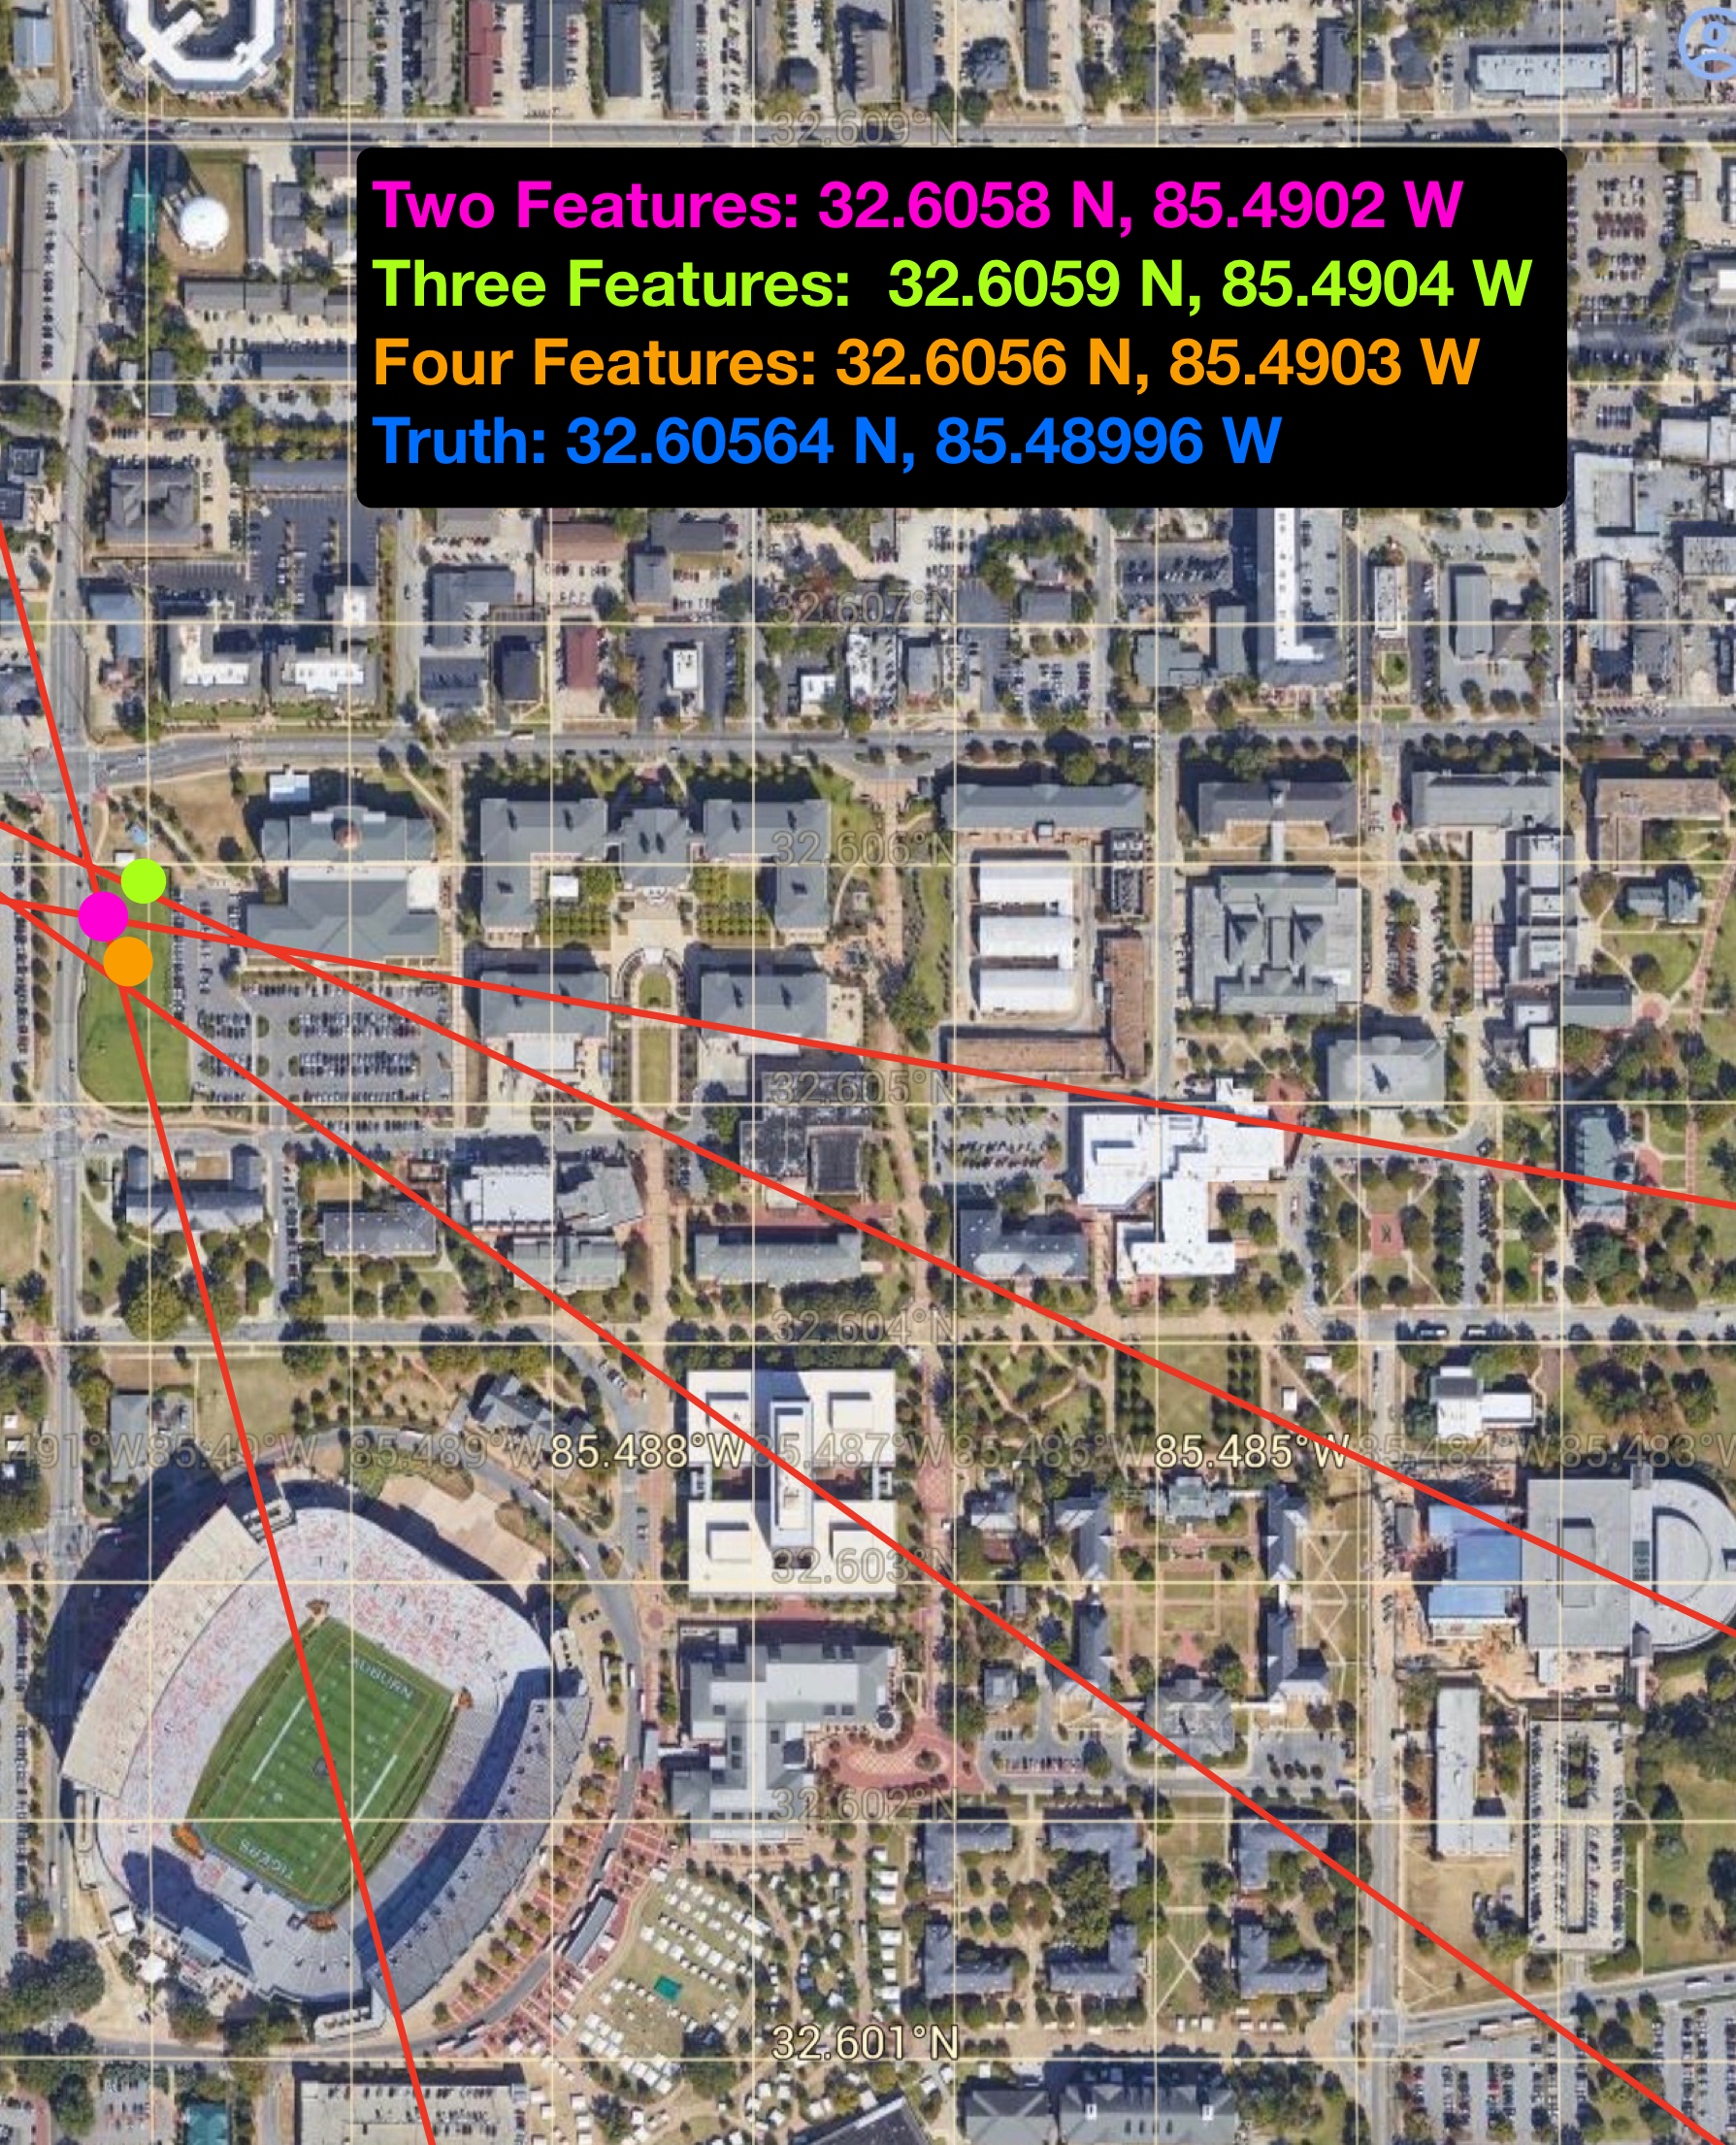
\includegraphics[width=\linewidth]{./figs/HW1_MAP.png}
        \caption{Position Triangulation Map}
        \label{fig:triPos}
    \end{figure}

    \clearpage

    \question
    Find and discuss a documented instance of a failure of navigation in a transoceanic flight. Be specific as to what went wrong and how this affected the mission.

    \solution
    Malaysia Airlines Flight 370 was a flight from Kuala Lumpur, Malaysia to Beijing, China that was mysteriously lost in the Southern Indian Ocean. The suspected reasons for this crash include a hypoxia event or possible hijacking, but do not directly blame a loss of reliable navigation. However, a navigation component on the aircraft failed and prevented the quick recovery of the crashed aircraft. Specifically, the transponder on the aircraft used by a secondary radar for air traffic control (ATC) failed or was turned off. This prevented critical aircraft state data from being transmitted to ATC which would've extremely helped the search for the lost plane. It's hard to say the crash would've been prevented, but the site would've likely been known and the plane would have been recovered. It turns out the search for the site continued for 4 years after the fact to no avail. If the transponder didn't fail, the cause of the crash would've likely been able to be determined.

    \clearpage

    \question
    Find and discuss a documented instance of a failure of guidance in a transoceanic
    flight. Be specific as to what went wrong and how this affected the mission.

    \solution
    American Airlines Flight 965 was a flight from Miami, FL to Cali, Colombia where the pilots mistakenly eliminated waypoints from their guidance system and attempted to reacquire them only to crash into a mountain in Buga, Colombia.

    Upon descent, the pilots of Flight 965 were asked if they wanted to use a non-precision approach to fly straight into a different runway than the one originally intended. The pilots accepted the offer as it would decrease the total flight time. In an attempt to clear the last few waypoints to their original runway, the pilots erroneously deleted all of their approach waypoints from the flight management system (FMS). This forced them to use a chart of waypoint stations to reprogram the waypoints into the FMS as they were approaching the airport. It just so happens the FMS did not follow the same naming convention as the chart and an incorrect waypoint was programmed in. Specifically, a waypoint that took the plane to Bogota. This caused the plane to turn and put them on a crash course with a mountain.

    The guidance system did its job very well, but the FMS database should've been changed to match the waypoint chart. This inherently places the guidance system at fault as the pilots could not have known they were reprogramming the FMS incorrectly until it was too late. The guidance system should've had checks in place to detect possible crash courses given the current navigation solution. However, this was unfortunately not the case. There were 159 fatalities among the 163 passengers and crew.

    \clearpage

    \question
    Assume that you have 1000 noisy biased measurements of the acceleration (scalar) of
    a stationary body over 100 seconds (i.e. $dt = 0.1$) as shown in the equation below.
    Numerically integrate the noisy biased measurements of acceleration to calculate
    “velocity” and “position” (assume zero initial conditions). Repeat this process 100
    times such that you have 100 random velocity and position values from each time
    step. Calculate the variance of the velocity and position at each time step and plot
    them versus time.

    \begin{equation}
        \begin{split}
            \tilde{\ddot{x}}& = \ddot{x} + b + \eta \\
            b& = 3 \\
            \eta&~\sim N(0,1)
        \end{split}
    \end{equation}

    \solution{A Monte Carlo simulation was run on integrated accelerometer values that contain bias and noise. The variance of the resulting velocities and positions are shown in Figures~\ref{fig:velVar} \&~\ref{fig:posVar}.

        \begin{figure}[!ht]
            \centering
            \includegraphics[width=\linewidth]{./figs/MC_VEL_RESULTS.png}
            \caption{Velocity Monte Carlo Results}
            \label{fig:velVar}
        \end{figure}

        \begin{figure}[!ht]
            \centering
            \includegraphics[width=\linewidth]{./figs/MC_POS_RESULTS.png}
            \caption{Position Monte Carlo Results}
            \label{fig:posVar}
        \end{figure}
    }

    \question{Given the simulated acceleration measurements for problem 5, how would you
        estimate the bias? Compute 100 estimates of the bias use each set of 1000
        measurements. What is the mean and variances of the bias estimates?}

    \solution{Given the body is known to be stationary, the bias can be calculated by
        determining the mean of the 1000 samples. The mean and variances of the bias estimates are shown below.

        \begin{equation*}
            \begin{split}
                \bar{\hat{b}} & = 2.998 \\
                \sigma^2(\hat{b}) & = 0.001 \\
                \sigma(\hat{b}) & = 0.029
            \end{split}
        \end{equation*}

    }
    \clearpage

    \question{You set out from town A and head east to town B 120 km away. Your vehicle has an
        odometer that is not particularly accurate (it could be off by 1-2 km after 50 km of
        driving). You carry a decent watch, which is great at keeping time over short
        intervals, but it has been months since you last reset it. In other words, you can
        measure time intervals accurately, but do not know exactly what time it is. A short
        time into your journey, the car breaks down.}

    \begin{parts}

        \part
        According to your odometer, you have traveled 56 km. Estimate your position.

        \solution
        My position estimate is 56 km from town A although there is a variance associated with the odometer after 50 km of travel. As the driver, I would only know what the odometer tells me and not the uncertainty associated with it.

        \part
        As you push your car to the shoulder of the road, a red bus zooms by heading
        from A to B. You glance at your watch and notice that it is exactly 21 minutes past
        the hour. You know that the red buses are prompt, and they leave town A every
        hour on the hour traveling at exactly 3 km/min. Can you estimate your position
        without using the odometer information?

        \solution{No, you cannot estimate it accurately. You could assume your position is 63 km from town A given $3~\si{km/min} \cdot 21~\si{min} = 63~\si{km}$; however, this assumption is invalid because your time is not accurate. You would need the odometer to estimate your clock bias which then allows you to accurately estimate your position.}

        \part
        Estimate your position and clock bias based on all the information so far (Hint:
        Write two equations that relate your position and clock bias to the available
        information. These equations are sometimes referred to as navigation equations).

        \solution
        \begin{equation}
            \begin{split}
                x & = \dot{x}_{red}(\delta t_{red} + b_{t})
            \end{split}
            \label{eq:redBus}
        \end{equation}

        \begin{equation}
            \begin{split}
                x & =  x_{odom}
            \end{split}
        \end{equation}

        \begin{equation*}
            \begin{split}
                b_t & = \frac{x_{odom}}{\dot{x}_{red}} -\delta t_{red} \\
                b_t & = \frac{56~\si{km}}{3~\si{\frac{km}{min}}} - 21~\si{min} \\
                b_t & = -2\frac{1}{3}~\si{min} \\
                x & = 3(21-2\frac{1}{3}) \\
                x & = 56 \si{km}
            \end{split}
        \end{equation*}

        It should be noted that the clock bias estimate has some uncertainty associated with it from the odometer that is not represented in the solution above. Therefore, the position solution is not completely accurate.

        \part
        At 25 minutes past hour by your watch, you observe a blue bus zoom past at 2.5
        km/min, going from B to A. Blue buses leave town B every hour on the hour
        promptly and drive to town A at a constant speed. Estimate your position and
        clock bias based on all the information so far.

        \solution
        It is ideal to only use the buses to estimate our position because all errors in their position are deterministic. The addition of the odometer will add uncertainty to the bias and position estimates given the noise on its measurement. If all 3 of our measurements had noise it'd be worthwhile to use the odometer and weight accordingly; however, the addition of the odometer will only degrade our estimates as they can be directly solved with the deterministic bus positions. Using Equations~\ref{eq:redBus} \&~\ref{eq:blueBus}, the clock bias and my position can be solved for.

        \begin{equation}
            \begin{split}
                x & = 120~\si{km} - \dot{x}_{blue}(\delta t_{blue} + b_t)
            \end{split}
            \label{eq:blueBus}
        \end{equation}

        \begin{equation*}
            \begin{split}
                \dot{x}_{red}(\delta t_{red} + b_{t}) & = 120~\si{km} - \dot{x}_{blue}(\delta t_{blue} + b_t) \\
                63~\si{km} + 3~\si{\frac{km}{min}}b_t & = 120~\si{km}-62.5~\si{km}-2.5{\frac{km}{min}}b_t \\
                b_t & = -1~\si{min} \\
                x & = 120 - 2.5(25+(-1)) \\
                x & = 60~\si{km}
            \end{split}
        \end{equation*}

        \part
        How would your solution be affected if your watch were exactly five minutes fast
        and all the clocks in town A and town B were running five minutes fast?

        \solution
        You would now have to estimate the clock biases of each town in addition to your clock bias. These new estimates would change Equations~\ref{eq:redBus} \&~\ref{eq:blueBus} to include town A and B's respective clock biases. The answer for this particular case would not change if these biases were known using the previous methodology, but that is no longer the case.

        \part
        Now suppose that your odometer never worked and the only vehicles you see are
        identical yellow cabs of carrier L1. These cabs leave town A every minute on the
        minute and travel exactly 1 km/min to town B. Can you estimate your position
        and clock error? Would it help if there were identical green cabs of carrier L2
        leaving town B every minute on the minute and traveling at 1 km/min to town A?
        Explain briefly.

        \solution
        No, you cannot estimate your position and clock bias because you would have no way of knowing how far the cab traveled to you or what time it left. You would only know the cab's speed. You would also only have 1 range measurement and two unknowns if you were even able to find your range.  It would not help if there was another one traveling the other way either as you need to know the number of cabs between you and a town to determine any range. The ambiguity in the number of cabs would not allow you to find either clock bias or position as you have no useable range ($\delta x$). If you were there when the first cabs started, you could count the number of cabs you see from the first carrier (time passed) before you see the first from the other carrier. This number multiplied by $1 \si{\frac{km}{min}}$ would give your distance from halfway between the towns and which cab you saw first would tell you which town you're closest to.

    \end{parts}

    \clearpage

\end{questions}
\end{document}